\documentclass[fleqn, a4paper, 11pt, oneside]{amsart}
\usepackage{exsheets, tasks}
\usepackage{amsmath, amssymb, amsthm} %standard AMS packages
\usepackage{marginnote} %marginnotes
\usepackage{gensymb} %miscellaneous symbols
\usepackage{commath} %differential symbols
\usepackage{xcolor} %colours
\usepackage{cancel} %cancelling terms
\usepackage{siunitx} %formatting units
\usepackage{tikz, pgfplots} %diagrams
\usetikzlibrary{calc, hobby, patterns, intersections}
\usepackage{graphicx} %inserting graphics
\usepackage{hyperref} %hyperlinks
\usepackage{datetime} %date and time
\usepackage{ulem} %underline for \emph{}
\usepackage{xfrac} %inline fractions
\usepackage{enumerate, enumitem} %numbered lists
\usepackage{float} %inserting floats

\newcommand\numberthis{\addtocounter{equation}{1}\tag{\theequation}} %adds numbers to specific equations in non-numbered list of equations

\newcommand{\AxisRotator}[1][rotate=0]{
	\tikz [x=0.25cm,y=0.60cm,line width=.2ex,-stealth,#1] \draw (0,0) arc (-150:150:1 and 1);%
} %rotation symbols on axes

\theoremstyle{definition}
\newtheorem{example}{Example}
\newtheorem{definition}{Definition}

\theoremstyle{theorem}
\newtheorem{theorem}{Theorem}

\newcommand{\curl}{\mathrm{curl\,}}

\makeatletter
\@addtoreset{section}{part} %resets section numbers in new part
\makeatother

\renewcommand{\thesubsection}{(\arabic{subsection})}
\renewcommand{\thesection}{(\arabic{section})}

%section headings on left
\makeatletter
\def\specialsection{\@startsection{section}{1}%
	\z@{\linespacing\@plus\linespacing}{.5\linespacing}%
	%  {\normalfont\centering}}% DELETED
	{\normalfont}}% NEW
\def\section{\@startsection{section}{1}%
	\z@{.7\linespacing\@plus\linespacing}{.5\linespacing}%
	%  {\normalfont\scshape\centering}}% DELETED
	{\normalfont\scshape}}% NEW
\makeatother

%forces newline after subsection
\makeatletter
\def\subsection{\@startsection{subsection}{3}%
	\z@{.5\linespacing\@plus.7\linespacing}{.1\linespacing}%
	{\normalfont\itshape}}
\makeatother

\settasks{counter-format = tsk[1].}

\SetupExSheets{solution/print = true}

%opening
\title
{
	Differential and Integral Calculus\\
	Assignment 8
}
\author
{
	Aakash Jog\\
	ID : 989323563
}
\date{\formatdate{28}{5}{2015}}

\begin{document}
	
\maketitle
%\setlength{\mathindent}{0pt}

\begin{question}
	Calculate the following integrals
	\begin{enumerate}
		\item
			$\iint\limits_{D} y \dif x \dif y$ where $D$ is the region bounded by the curves $y^2 = 4 + 4 x$, $y^2 = 4 - 4 x$, $y = 0$.\\
			Hint: Use the change of variables $u = 4 x$, $v = y^2$
		\item
			$\iint\limits_{D} y \dif x \dif y$ where $D$ is the region bounded by the curves $y = x$, $y = 3 x$, $x y = 1$, $x y = 3$.\\
			Hint: Use the change of variables $x = \frac{u}{v}$, $y = v$.
		\item $\iint\limits_{D} e^{\frac{x + y}{x - y}} \dif x \dif y$ where $D$ is the region in the fourth quadrant bounded by the lines $y = 0$, $x = 0$, $y = x - 1$, $y = x - 2$.
		\item $\int\limits_{0}^{2} \int\limits_{0}^{\sqrt{2 x - x^2}} \sqrt{x^2 + y^2} \dif y \dif x$.
	\end{enumerate}
\end{question}

\begin{solution}
	\begin{enumerate}[leftmargin = *]
		\item
			The curves $y^2 = 4 + 4 x$ and $y^2 = 4 - 4 x$ intersect at $(0,-2)$ and $(0,2)$.\\
			Therefore, $y \in [0,2]$.\\
			Let
			\begin{align*}
				u & = 4 x \\
				v & = y^2
			\end{align*}
			Therefore,
			\begin{align*}
				y^2 & = 4 + 4 x & \to &  & v & = 4 + u \\
				y^2 & = 4 - 4 x & \to &  & v & = 4 - u \\
				y   & = 0       & \to &  & u & = 0
			\end{align*}
			Therefore, as $y \in [0,2]$, $v \in [0,4]$.\\
			Therefore, the domain $D = \{ (x,y) | -\frac{y^2 - 4}{4} \le x \le \frac{y^2 - 4}{4} , 0 \le y \le 2 \}$ is transformed to $\Delta = \{ (u,v) | v - 4 \le u \le 4 - v , 0 \le v \le 4 \}$.\\
			The Jacobian is
			\begin{align*}
				J &=
					\begin{vmatrix}
						x_u & x_v \\
						y_u & y_v \\
					\end{vmatrix}\\
				\therefore \frac{1}{J} &=
					\begin{vmatrix}
						u_x & u_y \\
						v_x & v_y \\
					\end{vmatrix}\\
				&=
					\begin{vmatrix}
						4 & 0   \\
						0 & 2 y \\
					\end{vmatrix}\\
				&= 8 y\\
				\therefore J &= \frac{1}{8 y}
			\end{align*}
			Therefore,
			\begin{align*}
				\iint\limits_{D} y \dif x \dif y & = \iint\limits_{\Delta} y |J| \dif u \dif v                                       \\
                                                                 & = \int\limits_{0}^{4} \int\limits_{v - 4}^{4 - v} y \frac{1}{|8 y|} \dif u \dif v \\
                                                                 & = \int\limits_{0}^{4} \int\limits_{v - 4}^{4 - v} \frac{1}{8} \dif u \dif v       \\
                                                                 & = \frac{1}{8} \int\limits_{0}^{4} \left( 4 - v - v + 4 \right) \dif v             \\
                                                                 & = \frac{1}{8} \int\limits_{0}^{4} (8 - 2 v) \dif v                                \\
                                                                 & = \frac{1}{8} \left( 8 \cdot 4 - 4^2 \right)                                      \\
                                                                 & = 2
			\end{align*}
		\item
			\begin{figure}[H]
				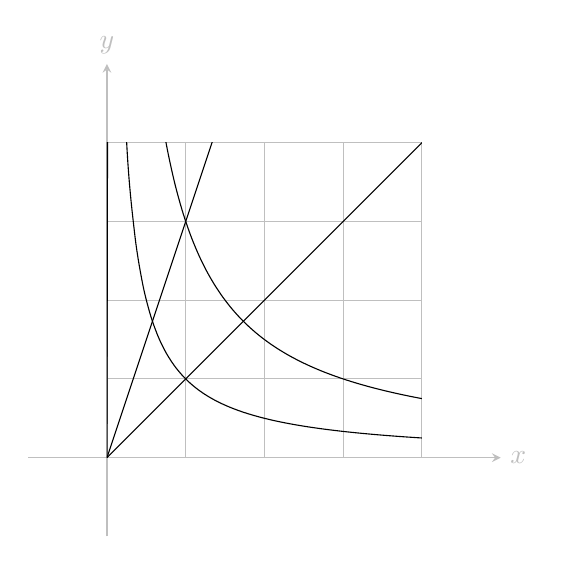
\begin{tikzpicture}
					\def\xMIN{-1};
					\def\xMAX{5};
					\def\yMIN{-1};
					\def\yMAX{5};

					\def\PI{22/7};

					\begin{scope}[lightgray]
						\draw [-stealth] (\xMIN,0) -- (\xMAX,0) node [right] {$x$};
						\draw [-stealth] (0,\yMIN) -- (0,\yMAX) node [above] {$y$};
						\draw (\xMIN + 1,\yMIN + 1) grid (\xMAX - 1,\yMAX - 1);
					\end{scope}

					\begin{scope}[smooth, samples = 100]
						\clip (\xMIN + 1,\yMIN + 1) rectangle (\xMAX - 1,\yMAX - 1);
						\draw plot (\x,\x);
						\draw plot (\x,3*\x);
						\draw plot (\x,1/\x);
						\draw plot (\x,3/\x);
					\end{scope}

					\begin{scope}
					\end{scope}
				\end{tikzpicture}
			\end{figure}
			Let
			\begin{align*}
				x & = \frac{u}{v} \\
				y & = v
			\end{align*}
			Therefore,
			\begin{align*}
				y            & = x   & \to &  & \frac{u}{v} & = v     \\
				\therefore y & = x   & \to &  & u           & = v^2   \\
				y            & = 3 x & \to &  & \frac{u}{v} & = 3 v   \\
				\therefore y & = x   & \to &  & u           & = 3 v^2 \\
				x y          & = 1   & \to &  & u           & = 1     \\
				x y          & = 3   & \to &  & u           & = 3
			\end{align*}
			Therefore, the Jacobian is
			\begin{align*}
				J &=
					\begin{vmatrix}
						x_u & x_v \\
						y_u & y_v \\
					\end{vmatrix}\\
				&=
					\begin{vmatrix}
						\frac{1}{v} & -\frac{u}{v^2} \\
						0           & 1              \\
					\end{vmatrix}\\
				&= \frac{1}{v}
			\end{align*}
			Therefore,
			\begin{align*}
				\iint\limits_{D} y \dif x \dif y & = \iint\limits_{\Delta} v |J| \dif u \dif v                                                 \\
                                                                 & = \iint\limits_{\Delta} v \cdot \frac{1}{v} \dif u \dif v                                   \\
                                                                 & = \int\limits_{1}^{3} \int\limits_{\sqrt{\frac{u}{3}}}^{\sqrt{u}} \dif v \dif u             \\
                                                                 & = \int\limits_{1}^{3} \sqrt{\frac{u}{3}} - \sqrt{u} \dif u                                  \\
                                                                 & = \left( \frac{1}{\sqrt{3}} - 1 \right) \int\limits_{1}^{3} \sqrt{u} \dif u                 \\
                                                                 & = \left( \frac{1}{\sqrt{3}} - 1 \right) \left. \frac{2}{3} x^{\frac{3}{2}} \right|_{1}^{3}  \\
                                                                 & = \left( \frac{1}{\sqrt{3}} - 1 \right) \left( \frac{2}{3} 3 \sqrt{3} - \frac{2}{3} \right) \\
                                                                 & = \left( \frac{1}{\sqrt{3}} - 1 \right) \left( 2 \sqrt{3} - \frac{2}{3} \right)
			\end{align*}
		\item
			Let
			\begin{align*}
				u & = x + y \\
				v & = x - y
			\end{align*}
			Therefore,
			\begin{align*}
				x & = 0     & \to &  & u & = -v \\
				y & = 0     & \to &  & u & = v  \\
				y & = x - 1 & \to &  & v & = 1  \\
				y & = x - 2 & \to &  & v & = 2
			\end{align*}
			Therefore, the Jacobian is
			\begin{align*}
				J &=
					\begin{vmatrix}
						x_u & x_v \\
						y_u & y_v \\
					\end{vmatrix}\\
				\therefore \frac{1}{J} &=
					\begin{vmatrix}
						u_x & u_y \\
						v_x & v_y \\
					\end{vmatrix}\\
				&=
					\begin{vmatrix}
						1 & 1  \\
						1 & -1 \\
					\end{vmatrix}\\
				&= -2
			\end{align*}
			Therefore,
			\begin{align*}
				\iint\limits_{D} e^{\frac{x + y}{x - y}} \dif x \dif y & = \iint\limits_{\Delta} e^{\frac{u}{v}} |J| \dif u \dif v                            \\
                                                                                       & = 2 \int\limits_{1}^{2} \int\limits_{-v}^{v} e^{\frac{u}{v}} \dif u \dif v           \\
                                                                                       & = 2 \int\limits_{1}^{2} \left. v e^{\frac{u}{v}} \right|_{-v}^{v}                    \\
                                                                                       & = 2 \int\limits_{1}^{2} \left( v e^{\frac{v}{v}} - v e^{\frac{-v}{v}} \right) \dif v \\
                                                                                       & = 2 \int\limits_{1}^{2} \left( v e - \frac{v}{e} \right) \dif v                      \\
                                                                                       & = 2 \left( e - \frac{1}{e} \right) \int\limits_{1}^{2} v \dif v                      \\
                                                                                       & = 2 \left( e - \frac{1}{e} \right) \frac{3}{2}                                       \\
                                                                                       & = 3 \left( e - \frac{1}{e} \right)
			\end{align*}
		\item
			\begin{align*}
				I & = \int\limits_{0}^{2} \int\limits_{0}^{\sqrt{2 x - x^2}} \sqrt{x^2 + y^2} \dif y \dif x
			\end{align*}
			Therefore,
			\begin{gather*}
				0 \le x \le 2 \\
				0 \le y \le \sqrt{2 x - x^2}
			\end{gather*}
			Therefore, the boundary is
			\begin{align*}
				y                          & = \sqrt{2 x - x^2} \\
				\therefore y^2             & = 2 x - x^2        \\
				\therefore x^2 + y^2 - 2 x & = 0                \\
				\therefore (x - 1)^2 + y^2 & = 1
			\end{align*}
			Therefore, the boundary is a circle with radius $1$, centred at $(1,0)$.\\
			Therefore, let
			\begin{align*}
				x - 1 & = r \cos \theta \\
				y     & = r \sin \theta
			\end{align*}
			Therefore,
			\begin{align*}
				\int\limits_{0}^{2} \int\limits_{0}^{\sqrt{2 x - x^2}} \sqrt{x^2 + y^2} \dif y \dif x & = \int\limits_{0}^{1} \int\limits_{0}^{2 \pi} r \cdot r \dif \theta \dif r \\
                                                                                                                      & = 2 \pi \int\limits_{0}^{1} r^2 \dif r                                     \\
                                                                                                                      & = 2 \pi \cdot \frac{1}{3}                                                  \\
                                                                                                                      & = \frac{2 \pi}{3}
			\end{align*}
	\end{enumerate}
\end{solution}

\begin{question}
	Calculate the area bounded by the curves $x = q y$, $x = p y$, $x y = b^2$, $x y = a^2$, where $q > p > 0$, $b > a > 0$.
\end{question}

\begin{solution}
	The boundaries are,
	\begin{align*}
		x                      & = q y \\
		\therefore \frac{x}{y} & = q   \\
		x                      & = p y \\
		\therefore \frac{x}{y} & = p   \\
		x y                    & = b^2 \\
		x y                    & = a^2
	\end{align*}
	Therefore, let
	\begin{align*}
		\frac{x}{y} & = u \\
		x y         & = v
	\end{align*}
	Therefore,
	\begin{align*}
		\frac{x}{y} & = q   & \to &  & u & = q   \\
		\frac{x}{y} & = p   & \to &  & u & = p   \\
		x y         & = b^2 & \to &  & v & = b^2 \\
		x y         & = a^2 & \to &  & v & = a^2
	\end{align*}
	Therefore, the Jacobian is
	\begin{align*}
		J &=
			\begin{vmatrix}
				x_u & x_v \\
				y_u & y_v \\
			\end{vmatrix}\\
		\therefore \frac{1}{J} &=
			\begin{vmatrix}
				u_x & u_y \\
				v_x & v_y \\
			\end{vmatrix}\\
		&=
			\begin{vmatrix}
				\frac{1}{y} & -\frac{x}{y^2} \\
				y           & x              \\
			\end{vmatrix}\\
		&= \frac{x}{y} + \frac{x}{y}\\
		&= 2 \frac{x}{y}\\
		\therefore J &= 2 \frac{y}{x}
	\end{align*}
	Therefore,
	\begin{align*}
		\left| \iint\limits_{D} \dif x \dif y \right| & = \left| \iint\limits_{\Delta} |J| \dif u \dif v \right|                                                \\
                                                              & = \left| \int\limits_{p}^{q} \int\limits_{a^2}^{b^2} \left| 2 \frac{y}{x} \right| \dif u \dif v \right| \\
                                                              & = \left| \int\limits_{p}^{q} \frac{1}{u} \dif u \int\limits_{a^2}^{b^2} \dif v \right|                  \\
                                                              & = \left| \left( \ln \frac{q}{p} \right) \left( b^2 - a^2 \right) \right|
	\end{align*}
\end{solution}

\begin{question}
	The change of variables
	\begin{align*}
		x & = u + 2 v + 1 \\
		y & = 2 u + v + 1
	\end{align*}
	maps the unit circle $u^2 + v^2 \le 1$ to a region $D$ in the $x$-$y$ plane.
	\begin{enumerate}
		\item Find the area of $D$.
		\item 
			Let $R$ be some region in the $u$-$v$ plane and let $D$ be its image in the $x$-$y$ plane under the above change of variables.
			Prove that $\mathrm{Area}(D) = 3 \mathrm{Area}(R)$.
		\item
			Let
			\begin{align*}
				x &= \varphi(u,v)\\
				y &= \psi(u,v)
			\end{align*}
			be some other change of variables from the $u$-$v$ plane into the $x$-$y$ plane, where $\varphi$, $\psi$ are one-to-one, $C^1$ functions for which there exist $M > 0$, such that for every point in the $u$-$v$ plane, the following inequalities are satisfied
			\begin{align*}
				|\varphi_u| & \le M \\
				|\varphi_v| & \le M \\
				|\psi_u|    & \le M \\
				|\psi_v|    & \le M
			\end{align*}
			Let $R$ be a region in the $u$-$v$ plane and let $D$ be its image under the above change of variables.
			Prove that $\mathrm{Area}(D) \le 2 M^2 \cdot \mathrm{Area}(R)$.
	\end{enumerate}
\end{question}

\begin{solution}
	\begin{enumerate}[leftmargin = *]
		\item
			\begin{align*}
				x & = u + 2 v + 1 \\
				y & = 2 u + v + 1
			\end{align*}
			Therefore, the Jacobian is
			\begin{align*}
				J &=
					\begin{vmatrix}
						x_u & x_v \\
						y_u & y_v \\
					\end{vmatrix}\\
					\begin{vmatrix}
						1 & 2\\
						2 & 1\\
					\end{vmatrix}\\
				&= -3\\
			\end{align*}
			\begin{align*}
				\iint\limits_{D} \dif x \dif y & = \iint\limits_{\Delta} |J| \dif u \dif v                                                             \\
                                                               & = \iint\limits_{\Delta} 3 \dif u \dif v                                                               \\
                                                               & = \int\limits_{-1}^{1} \int\limits_{-\sqrt{1 - u^2}}^{\sqrt{1 - u^2}} 3 \dif v \dif u                 \\
                                                               & = 3 \int\limits_{-1}^{1} \left( \sqrt{1 - u^2} + \sqrt{1 - u^2} \right) \dif u                        \\
                                                               & = 6 \int\limits_{-1}^{1} \sqrt{1 - u^2} \dif u                                                        \\
                                                               & = 6 \left( \left. \frac{1}{2} \left( \sqrt{1 - u^2} u + \sin^{-1}(u) \right) \right) \right|_{-1}^{1} \\
                                                               & = 3 \left( \sin^{-1} 1 - \sin^{-1} -1 \right)                                                         \\
                                                               & = 3 \left( \frac{\pi}{2} - \frac{-\pi}{2} \right)                                                     \\
                                                               & = 3 \pi
			\end{align*}
		\item
			\begin{align*}
				x & = u + 2 v + 1 \\
				y & = 2 u + v + 1
			\end{align*}
			Therefore, the Jacobian is
			\begin{align*}
				J &=
					\begin{vmatrix}
						x_u & x_v \\
						y_u & y_v \\
					\end{vmatrix}\\
					\begin{vmatrix}
						1 & 2 \\
						2 & 1 \\
					\end{vmatrix}\\
				&= -3\\
			\end{align*}
			\begin{align*}
				\mathrm{Area}(D) & = \iint\limits_{D} \dif x \dif y     \\
                                                 & = \iint\limits_{R} |J| \dif u \dif v \\
                                                 & = |J| \iint\limits_{R} \dif u \dif v \\
                                                 & = 3 \iint\limits_{R} \dif u \dif v   \\
                                                 & = 3 \cdot \mathrm{Area}(R)
			\end{align*}
			\qed
		\item
			\begin{align*}
				x & = \varphi(u,v) \\
				y & = \psi(u,v)
			\end{align*}
			Therefore, the Jacobian is
			\begin{align*}
				J &=
					\begin{vmatrix}
						x_u & x_v \\
						y_u & y_v \\
					\end{vmatrix}\\
				&=
					\begin{vmatrix}
						\varphi_u & \varphi_v \\
						\psi_u    & \psi_v    \\
					\end{vmatrix}\\
				&= \varphi_u \psi_v - \varphi_v \psi_u
				\intertext{Therefore, as $|\varphi_u| \le M$, $|\varphi_v| \le M $ $|\psi_u| \le M$, $|\psi_v| \le M$,}
				J &\le M^2 + M^2\\
				\therefore J &\le 2 M^2
			\end{align*}
			Therefore,
			\begin{align*}
				\mathrm{Area}(D)            & = \iint\limits_{D} \dif x \dif y     \\
                                                            & = \iint\limits_{R} |J| \dif u \dif v \\
                                                            & = |J| \iint\limits_{R} \dif u \dif v \\
                                                            & = |J| \mathrm{Area}(R)               \\
				\therefore \mathrm{Area}(D) & \le |2 M^2| \mathrm{Area}(R)         \\
				\therefore \mathrm{Area}(D) & \le 2 M^2 \mathrm{Area}(R)           \\
			\end{align*}
			\qed
	\end{enumerate}
\end{solution}

\end{document}
